%
% File: chap03.tex
% Author:
% Description: Design and Implementations
%
\chapter{Design and Implementations}
\label{chap:D&I}

Begins a chapter. Example: When the beloved cellist (Christopher Walken - outstanding) of a world-renowned string quartet receives a life-changing diagnosis, the group's future suddenly hangs in the balance: suppressed emotions, competing egos and uncontrollable passions threaten to derail years of friendship and collaboration. Featuring a brilliant ensemble cast (including Philip Seymour Hoffman, Catherine Keener and Mark Ivanir as the three other quartet members), it is a fascinating look into the world of working musicians, and an elegant homage to chamber music and the cultural world of New York. The music, of course, is ravishing (the score is the work of regular David Lynch collaborator Angelo Badalamenti): A Late Quartet hits all the right notes.

\section{Methodology}
\label{sec:sec01}

\subsection{Work Flow}
\label{subsec:subsec01}

\subsection{Front-end Tools}
\label{subsec:FETools}
%
% File: chap03-01-02.tex
% Author: 
% Description: 
% 3.1 Methodology
%  3.1.2 Front-end Tools
%     Figma
%     HTML
%     CSS
%     SpringBoot+Thymeleaf
%

\paragraph{Figma}\mbox{}\\
In our project, our goal is to design a website for medical use. As a team, we all agree that a high-quality website should include several essential factors. Among them, user interface (UI) and user experience (UX) are the most crucial. A well-designed website should maintain a consistent and visually appealing style across all pages, while also being intuitive to use and free from confusing workflows. Another key consideration is the design process itself. Since we are working as a team, it is important to choose a tool and workflow that supports efficient collaboration. First, team members should be allowed to work independently or collaboratively while still ensuring consistency across design. Second, we need a real-time collaborative environment to prevent any individual’s progress from being delayed by others. 

For achieving our project goals, we evaluate two tools, Canva and Figma. Both are useful for collaborative website development and support real-time commenting to improve teamwork. However, the key differences lie in several areas. First is layout design. Figma allows for the detailed design of every element on each page, including font size and CSS box models. In contrast, Canva cannot adjust all elements individually and focuses more on overall visual design. Second is interactive prototyping. Figma features in demonstrating the website’s workflow by allowing us to define the behavior of elements like buttons and links to fully simulate the website experience. Canva, on the other hand, can only create simple links between pages. Third is version control. Figma automatically records a comprehensive history of all changes, while Canvas offers relatively basic version control functions. Ultimately, Figma is our final choice for this project because it provides all the features we need for professional web development.

As our final decision, Figma improved our work due to these features:
\begin{itemize}
    \item \textbf{Real-time Collaboration and Efficiency}: Figma enabled us to work simultaneously in the cloud, with live editing and immediate feedback eliminating unnecessary back-and-forth communication. This transparency allowed everyone to see ongoing progress, making it easier to coordinate tasks and iterate on designs much faster.
    \item \textbf{Guaranteed Visual Consistency}: By utilizing shared elements, colors, and font styles, we successfully maintained a coherent and consistent visual language across the entire interface.
    \item \textbf{Streamlined Development Handoff}: One of the most practical benefits was the automatic generation of CSS code for design properties. This feature greatly enhanced our efficiency by simplifying the process of translating designs into front-end code.
    \item \textbf{Clear Accountability and Version Control}: The ability to tag team members in comments kept us aligned on assigned sections. Furthermore, the comprehensive version control function provided a clear history of all changes, ensuring accountability and allowing us to review progress at any stage.
    \item \textbf{Fostered Collaborative Ownership}: Ultimately, Figma didn't just reduce confusion and latency; it fostered a strong sense of shared ownership over the design. It ensured that our team worked as a cohesive unit, building a product with a unified vision.
\end{itemize}

\paragraph{HTML}\mbox{}\\
We aim to provide a clean, accessible and responsive interface for medical users. To achieve this goal, we requires tools that help us build structured, semantic layouts while maintaining visual consistency across devices and screen sizes. When evaluating which front-end tools were most suitable for our design, we considered several combinations, including HTML with Bootstrap, HTML with TailwindCSS, and SCSS-based modular design systems. According to the specific characteristics of our project and our situation. We all agree that using HyperText Markup Language(HTML) and Cascading Style Sheets(CSS) was the most appropriate choice for our needs after discussion. In the following section, we provide a brief introduction to these two technologies and explain how they contributed to the development of our prototype.

HTML is a necessary and standard core language that can be interpreted by any modern web browsers. In web development, HTML is used to arrange the content of the website and provide basic structural syntax for page design. As a fundamental tool, HTML has a relatively simple and easy-to-learn syntax, allowing developers to create websites with clear semantic structures that enhances both accessibility and user-friendliness. HTML wild ranges of labels, such as \verb|<head>|, \verb|<p>|, and \verb|<div>|, which are used to organise the layout of a page. These elements support essential functions like hyperlinks, image embedding, list creation and tables formatting. With just basic syntax, developers can easily achieve a certain level of responsive functionality. Although various tools exists to assist in web development—such as page builders or frameworks—all of them ultimately compile down to HTML. As a result, HTML is irreplaceable in the front-end development process. Due to the situation our team has encountered, we all agree that the cost of learning alternative tools would beyond their benefits. Therefore, we decide to directly use plain HTML as our primary front-end tool. However, as mentioned above, HTML only provides basic structure and limiting styling capabilities. Managing layout and appearance directly within HTML would lead to inefficiencies and inconsistency. To address this issue, we employed CSS to handle visual design and layout, which will be discussed in next section. 

\paragraph{CSS}\mbox{}\\
One crucial issue in web development is how to manage code efficiently and make it maintainable. A widely adopted and effective solution is to separate the content, functionality and the style into distinct layers. While tools such as SCSS, Tailwind CSS and Bootstrap provide advanced styling features, we ultimately chose to use standard CSS for this project. This decision was based on the simplicity and clarity that CSS provides--especially valuable for a small team working on a focused prototype. CSS allows us to directly translate our Figma designs into code without introducing additional syntax or dependencies. This made it easier for all team members to understand and contribute to the styling process. Besides, one of the key advantages of CSS is its clear separation of content and presentation, which improves maintainability and enables us to update visual styles without modifying the fundamental structure. CSS also plays a crucial role in transforming our HTML structure into a clean, professional, and user-friendly interface. Furthermore, CSS enhances our collaboration by allowing us to define a shared layout and style system. Each members can easily apply consistent styles across pages, significantly reducing time spent on detail adjustments, and improving the efficiency of our workflow.

\paragraph{Spring Boot and Thymeleaf}\mbox{}\\
Before selecting our technology stack for the Smart Hospital web application, we weighed a number of backend and frontend framework possibilities with consideration of equating development speed, maintainability, and integration efficiency. The top contenders included Spring Boot with Thymeleaf, Node.js with Express and React, and Django with HTML templates. Table~\ref{tab:3-1-2-SBtable} summarizes the strengths and weaknesses of each stack based on thoroughly documented pros and cons according to credible sources.

\begin{table}[H]
  \centering
  
\includegraphics[width=0.8\linewidth]{images03/3-1-2-springbootTable.png} 
  \caption{Technology Stack Alternatives Comparison}
  \label{tab:3-1-2-SBtable}
\end{table}

We weighed these options and opted to go with Spring Boot in the backend and Thymeleaf in the frontend. This Java-focused stack provided us with a consistent and streamlined development environment, which was particularly crucial for our small team of individuals working on tight deadlines. Because both frameworks are based on the Java ecosystem, we were able to build full-stack functionality in one integrated project. This reduced the complexity that would have otherwise been caused by having two separate frontend and backend codebases and improved coordination among team members.\cite{Simplilearn-Nodejs-SB}

Spring Boot is a well-used enterprise-level framework that streamlines Java web application development. It provides an embedded Tomcat server, auto-configuration, and dependency management, allowing us to concentrate on core functionality instead of boilerplate setup.\cite{GFG-Djanggo-SB} Its innate RESTful API support enabled us to plan a scalable, modular backend architecture, with Controller classes as the basis for API endpoints, a core feature for connecting the client interface to backend services.

At the frontend, Thymeleaf was selected as a server-side templating engine that has native support for Spring Boot's MVC framework. Its dynamic binding of backend data in HTML templates ensured tight coupling of presentation logic with backend processes. This eliminated the need for extra JavaScript frameworks like React or Angular, reducing the learning curve and allowing the team to progress faster. Thymeleaf's human-readable syntax also made collaboration easier and the codebase more maintainable.\cite{JavaGuides-Thymeleaf-ReactJS}

Alternatives such as Node.js with Express and React were also considered, which would have offered highly interactive UIs and would have leveraged JavaScript's extensive ecosystem, but would also have meant two codebases to manage and deployment complexity.\cite{Simplilearn-Nodejs-SB} Django with HTML templates, knowingly able to achieve rapid development and secure by design \cite{GFG-Djanggo-SB}, was also a consideration but would have required the team to learn Python, an undesirable learning curve considering the time constraints we had.

Finally, our academic supervisor recommended picking up Spring Boot with Thymeleaf for its combination of performance, integration ease, and suitability for a Java-experienced team. This also simplified deployment, as both backend and frontend could be deployed together in a single application. Moving further to the backend implementation phase, Spring Boot Controller classes will accept incoming HTTP requests and will form the basis of our API layer, which, later on, will be tested by tools discussed in the Backend Tools section.


\subsection{Back-end Tools}
\label{subsec:subsec04}

\subsection{Testing Tools}
\label{subsec:subsec05}

\section{Front-end Design and Implementations}
\label{sec:sec02}

\subsection{Early Stage-Virtual Hospital Africa(VHA)}
\label{subsec:subsec01}

During the initial discussions with the client, it was identified that the \textbf{Patient Intake page}
contained too many information fields. This led to poor user experience, with many testers
abandoning the form midway (Figure~\ref{fig:intake1}).
To address this, the client designed a second version of a multi-step form interface (Figure~\ref{fig:intake2}).
Finally, after our team's feedback, a third version was created (Figure~\ref{fig:intake3}).

\subsubsection{Key Improvements in Patient Intake Page}
\begin{enumerate}
    \item \textbf{Left-side navigation bar:} Enabled non-linear navigation, allowing users to jump to
    any section freely, improving flexibility and control.
    \item \textbf{Optimized field grouping:} Consolidated fields such as name, gender, title, language,
    and ID number into a ``General'' group. Added profile photo upload with instant preview.
    \item \textbf{Unified navigation buttons:} Replaced inconsistent buttons with clear
    \emph{Back/Next}, improving predictability and reducing disorientation.
\end{enumerate}

\subsubsection{Patient Profile Page Improvements}
\begin{enumerate}
    \item \textbf{Enhanced patient information card:} Added profile picture, gender/age tags, patient status,
    quick contact and download buttons, and last edit time.
    \item \textbf{Expanded information modules:} Unified the top tab bar and added a secondary menu
    (General, Primary Care, Contacts, Biometrics, Insurance).
    \item \textbf{Editable forms:} Personal data presented in structured fields supporting direct editing.
\end{enumerate}

\subsubsection{Vitals Page Redesign}
\begin{enumerate}
    \item \textbf{Grouped layout:} Divided vital signs into ``Required'' and ``Optional'' sections,
    aligning with clinical practices.
    \item \textbf{Optimized workflow:} Replaced single ``Continue'' button with \emph{Back/Next},
    allowing users better control.
    \item \textbf{Integration with patient panel:} Displayed patient summary and treatment timeline
    alongside data entry.
\end{enumerate}

These improvements adhered to usability principles such as
\emph{Match between system and the real world},
\emph{Visibility of system status}, and
\emph{Recognition rather than recall},
reducing cognitive load, improving efficiency, and minimizing errors.



\subsection{Smart Hospital}
\label{subsec:subsec02}
%
% File: chap03-02-02.tex
% Author:
% Description:
% 3.2 Front-end Design & Implementation
%  3.2.1 Smart Hospital
%     Design Process
%     Front-end Implementation
%

\paragraph{Design Process}\mbox{}
\paragraph{From Concept to User Needs: Ideation and Story Mapping}\mbox{}\\
After the basic requirements in Section 2.3 were written, the next step was to think about how the Smart Hospital could really work in practice. Because the main goal of the system is to solve the problem of many local residents not getting proper treatment, the design started from the patient’s side, thinking about what kind of functions they may need.

Next, some existing problems in hospitals were analysed. Two team members with hospital internship experience observed many issues in real hospitals. For example, nurses often record patient information by hand. In some cases, the writing is messy, so it is hard to read or may cause mistakes. It also takes time to find previous records, and paper files may be lost. Patients face several problems when they try to get their medical history as well. They often have to fill in a lot of forms and wait for a long time in hospitals. Sometimes the staff cannot even find the records among the large number of paper documents, which is inconvenient for both patients and hospitals.
The background of the Virtual Hospital Africa system was also considered. In South Africa, medical resources are not well distributed. Many people in rural areas need to travel a long distance to big hospitals if they want to see a doctor. At the same time, some people go to the hospital even for small problems that might not need to go to a hospital, but they don’t know what to do. This situation makes the hospital more crowded. If these problems can be solved by an online system, the efficiency will be much better.

Then, the tasks of each role were listed. Patients want to have online consultations, ask health questions, and download their reports. Nurses want to input vitals like blood pressure and temperature using computers. Doctors want to review patient history, record diagnoses, and give prescriptions. All of these were written into user stories, some of which are shown in Table 2.1.

For each user story, we used the method we learned in the Software Engineering Discipline and Practice class — Planning Poker — to evaluate the technical difficulty. As shown in Figure~\ref{fig:planning_poker_examples}, we used the Fibonacci numbers 1, 2, 5, 8, 13, 21, and 34 as the scores so that the gap between the numbers was not too small; otherwise, the scores would not be meaningful. Each team member gave an individual score; then the stories with large differences were discussed, and a final agreement was reached. The simpler functions were implemented first, while the more complex ones were scheduled for later. In this way, the development had a clear order, and we did not get stuck at the beginning. We also kept updating the stories because the remaining time was limited, so it was necessary to ensure they were truly necessary.

\begin{figure}[h]
   \centering
   \begin{subfigure}[t]{0.45\textwidth}
     \centering
     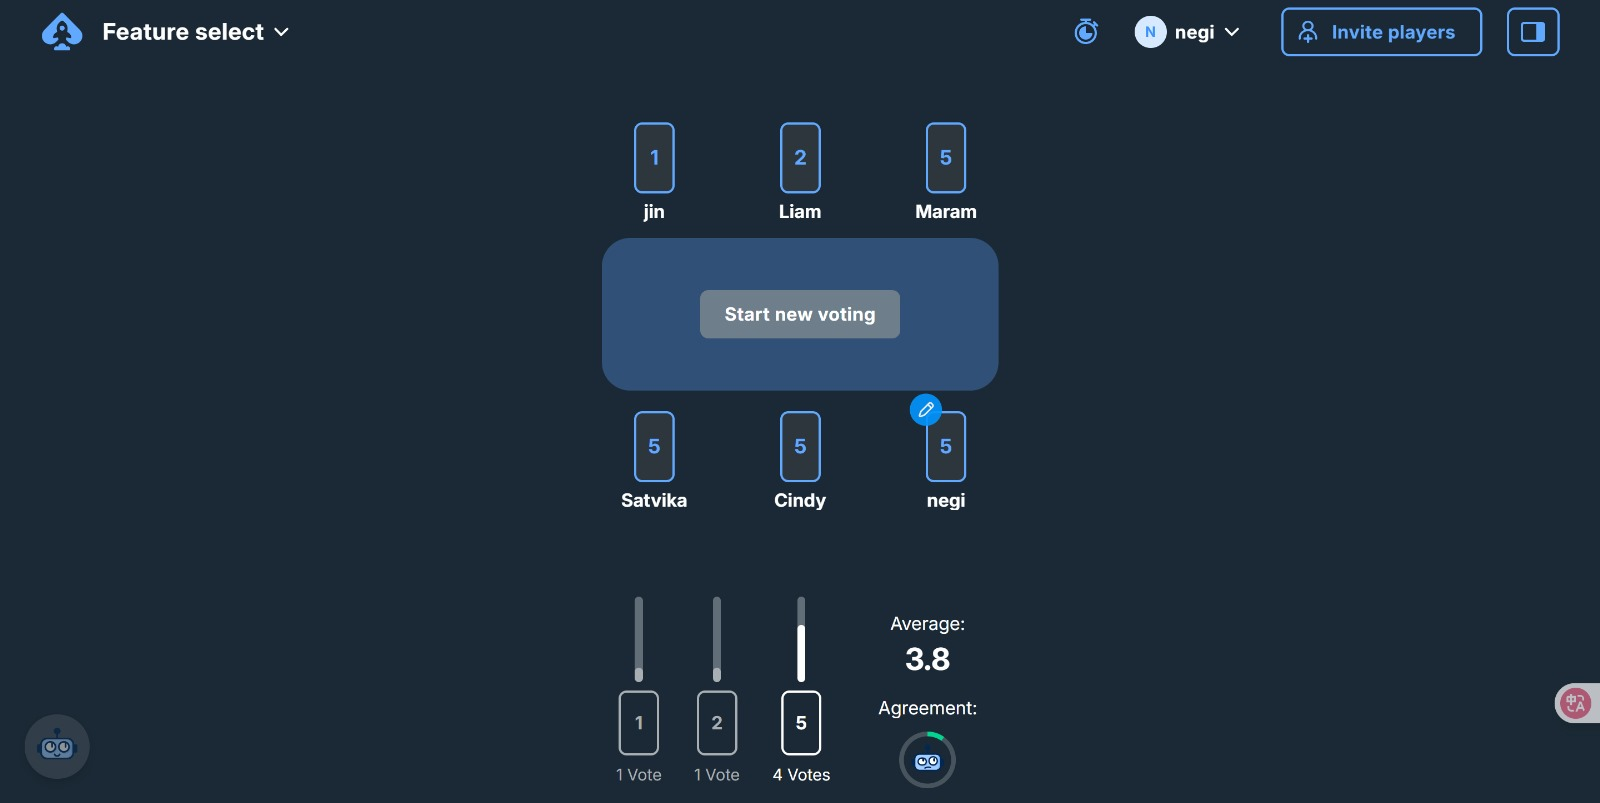
\includegraphics[width=\linewidth]{../../images/planning_poker_low.jpeg}
     \caption{Planning Poker result for the task "doctor records diagnoses," with an average score of 3.8.}
   \end{subfigure}%
   \hfill
   \begin{subfigure}[t]{0.45\textwidth}
     \centering
     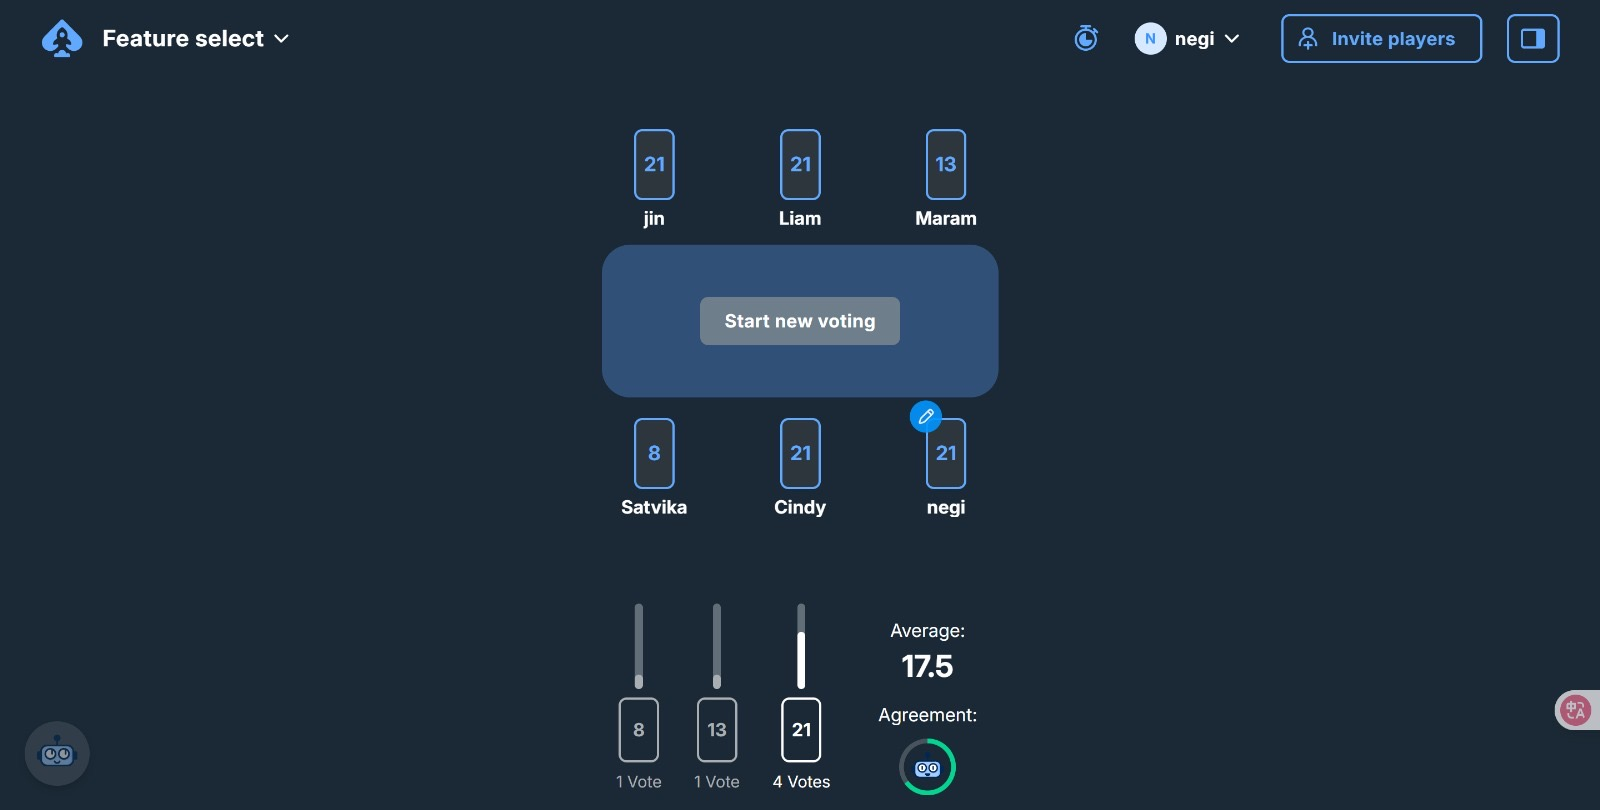
\includegraphics[width=\linewidth]{../../images/planning_poker_high.jpg}
     \caption{Planning Poker result for the task "Health Q\&A," with an average score of 17.5.}
   \end{subfigure}
   \caption{Examples of Planning Poker voting results.}
   \label{fig:planning_poker_examples}
\end{figure}

\paragraph{Bridging Stories and Systems: Workflow Design}\mbox{}\\

After writing the user stories, we started thinking about how these functions could actually connect with each other. For example, if a nurse records the patient’s blood pressure, the doctor should be able to see this data at the next visit. When the doctor checks the medical history and writes the diagnosis, the patient can then see the advice given by the doctor, and so on.

To make these workflows clearer, we drew user flow diagrams in Figma to show the paths of different roles in the system. As shown in Figure~\ref{fig:userflow-registration}, we began with the most basic authentication process, including login, registration, and password reset, so that all users can access the system.

\begin{figure}[H]
   \centering
   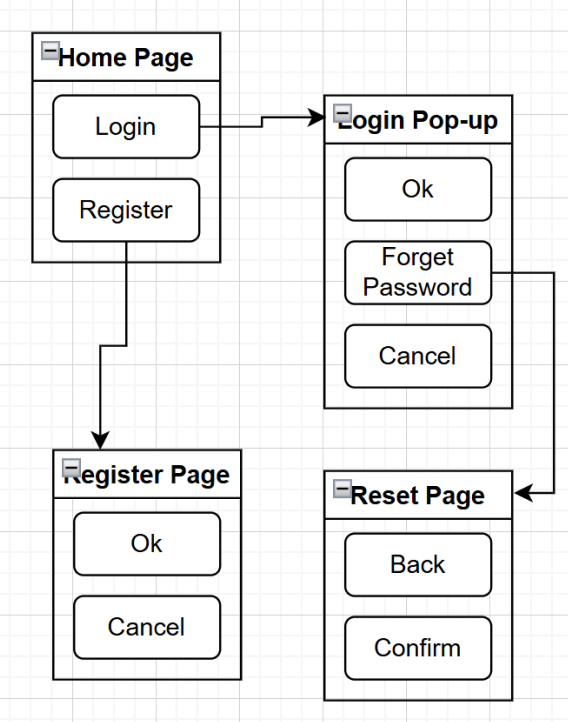
\includegraphics[width=0.4\linewidth]{../../images/userflow_registration.png}
   \caption{User flow diagram for the registration process.}
   \label{fig:userflow-registration}
\end{figure}

Next, we designed the main workflow for the patient role, as shown in Figure~\ref{fig:userflow-whole}. Starting from the dashboard, the patient can use the sidebar to navigate to different pages, including patient intake, patient profile, vital records, and prescriptions. Each page also contains the sidebar and a log-out option, so that the user can switch between functions and log out at any time.
\begin{figure}[H]
   \centering
   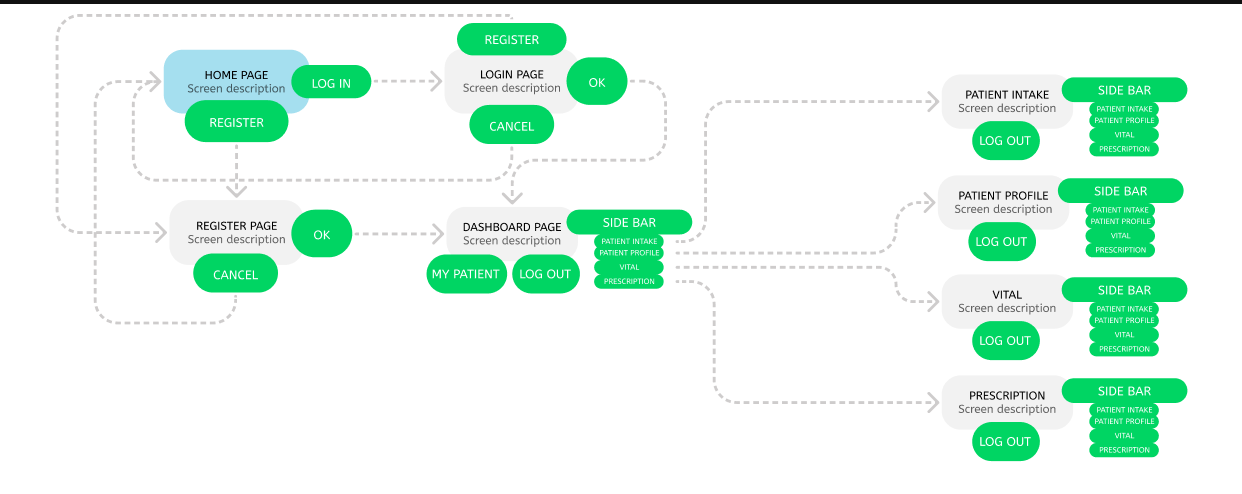
\includegraphics[width=1.1\linewidth]{../../images/userflow_whole.png}
   \caption{Overall user flow diagram of the system.}
   \label{fig:userflow-whole}
\end{figure}


For the function design on each role side, we followed how real hospitals usually work.
Patients can only see their own records and cannot see other people’s information.
For now, nurses can only enter vital signs.
Doctors have the most functions: they can view the full medical history and write diagnoses,
but they cannot change the patient’s basic information.
This setup is similar to how real hospitals operate. 

One difference from real hospitals is that we also considered the remote consultation process.
After the patient makes an appointment, they can first see the doctor from home.
If the doctor thinks it is needed, the patient will then go to a clinic to measure vital signs
or go to the hospital for further treatment.
This can reduce unnecessary visits, and at the same time, still make sure we do not miss any patients who really need care.

The user flow diagrams we drew in Figma helped us make sure each function connects smoothly,
and they also gave the frontend team a clear reference for page navigation.
At this stage, we clarified the logic of the hospital side.
For example, the user must log in before entering the dashboard,
and from the dashboard, they can directly or indirectly access all the designed pages.
These two basic user flow diagrams gave us a clear direction when we started designing the webpages.

\paragraph{Visualizing Functionality: Prototyping with Figma}\mbox{}\\
After we completed the workflow diagram, we used it as the foundation to divide tasks among team members. Each member is responsible for designing specific pages for different parts of the website while working all within a single file, shown as Figure~\ref{fig:3-2-2-DS-figma-f1}, simplified cross-reviewing and allowed for seamless handoffs instead of manually sending assets or screenshots . Next, we will introduce our layout design.
\begin{figure}[H]
  \centering
  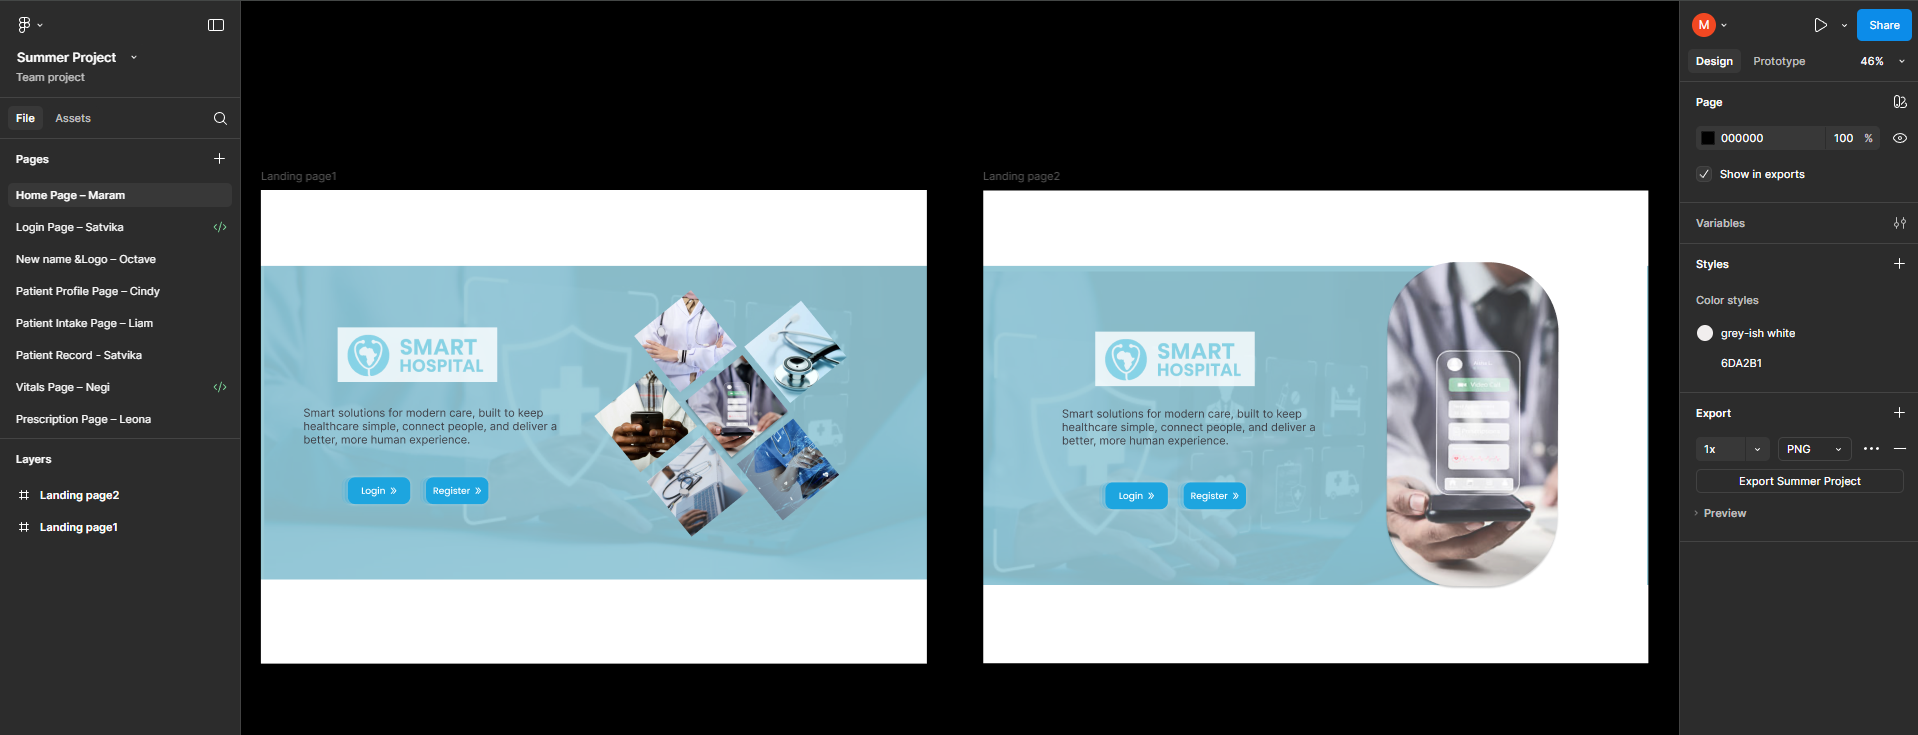
\includegraphics[width=0.8\linewidth]{images03/3-2-2-figure1.png}
  \caption{Shared Figma file displaying landing pages by Maram.}
  \label{fig:3-2-2-DS-figma-f1}
\end{figure}

The primary goal of our layout is to ensure intuitive user interaction. For example when doctors are diagnosing a patient, they typically start by reviewing the patient’s profile to gain a comprehensive understanding of the patient’s condition. This information is displayed on the “Patient Profile” page. At the same time, doctors may need access to the patient’s visits history, so we design a clear and concise list that displays the date of each visit, a brief summary of the diagnosis, and the attending physician. If more detailed information is needed, doctors can click the “view” button to open a pop-up window showing the full report. Another example is during the diagnosis process–doctors may want to take temporary notes before writing the final prescription or summary. To support this, we included a text area on the “Clinical Notes” page where doctors can write their notes down. These features are all designed to enhance the experience for medical professionals interacting with our platform.

Color selection plays a vital role in website design. In our project, we choose a range of blue tones as the primary color scheme, as blue often represents inclusiveness and trust. To make the overall atmosphere feel more approachable and friendly, we incorporate some earthy tones into the blue. Meanwhile, white and gray is used for  elements like buttons and text areas to create a clean and orderly appearance. Through these color combinations, we aim to convey a sense of stability and warmth to our users. The overall visual design reflects the spirit of our platform, to serve as a strong and trustworthy support for users of all ages, genders, physical conditions and cultural background.

We continually review each other’s work using the comment feature which is one of the most useful features we employed, to ensure real-time feedback and update.Throughout the development of each screen, we actively left comments for one another, either suggesting improvements or pointing out issues to be addressed. These comments were visible directly on the relevant design elements, helping us avoid miscommunication and track suggested changes efficiently.

We often initiated discussions either directly within Figma or first during our meetings, and then documented the agreed-upon feedback using the comment feature to ensure accountability. This helped prevent any feedback from being forgotten and gave each designer a clear to-do list for updates. For instance, comments could be left directly on the design (Figure~\ref{fig:figma-comments-example-direct}) or used to track resolved issues after a meeting (Figure~\ref{fig:figma-comments-example-direct-afmeetings}).
\begin{figure}[htbp]
  \centering
  \captionsetup[subfigure]{labelformat=simple, labelsep=space, justification=centering}
  \renewcommand{\thesubfigure}{(\alph{subfigure})}
  \begin{subfigure}[t]{0.48\linewidth}
    \centering
    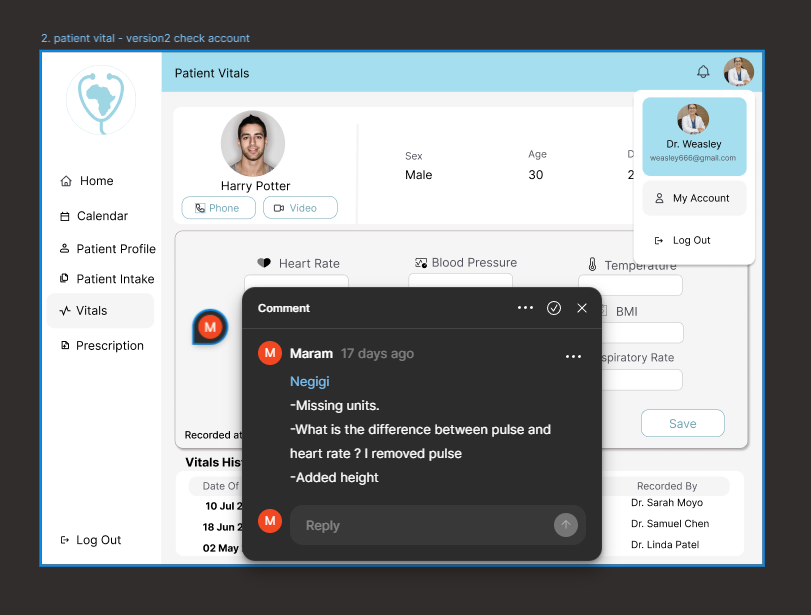
\includegraphics[height=6cm]{images03/3-2-2-figure2.png}
    \caption{Providing feedback via comments.}
    \label{fig:figma-comments-example-direct}
  \end{subfigure}\hfill
  \begin{subfigure}[t]{0.48\linewidth}
    \centering
    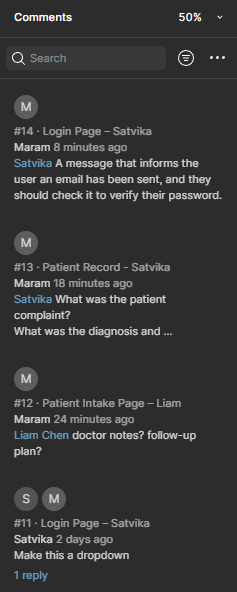
\includegraphics[height=6cm]{images03/3-2-2-figure3.png}
    \caption{Tracking and resolving design feedback.}
    \label{fig:figma-comments-example-direct-afmeetings}
  \end{subfigure}
  \caption{Using Figma's comment feature for collaborative design reviews.}
  \label{fig:figma-collaboration-comments}
\end{figure}

To evaluate whether the designs meet our requirements, we test various user scenarios using Figma’s prototyping feature to link different steps and assess the overall flow. Also, we shared links to Figma with our academic supervisor during our weekly review sessions so that they could view the prototype live. During these review sessions, we made use of the "Follow" feature so that we were all concentrated on the same element of the design so that it was simpler for the supervisor to provide targeted, contextual feedback on specific areas.

This direct communication also allowed us to quickly clarify and allowed us to reduce uncertainty about comments such as "this needs to be more visible" or "consider redesigning this layout."

Moreover, Figma’s version history feature allowed us to continuously improve our design by reflecting on what worked and what didn’t. Although we didn’t manually take snapshots, Figma automatically saved our progress, which made it easy to revisit previous versions at any point. This proved especially helpful when comparing earlier designs with more refined iterations, as it allowed us to clearly see what had improved and what needed further adjustment.

A great example of this is the evolution of the Vitals page, which went through at least six major visual and functional changes, shown in Figure~\ref{fig:vitals-evolution}. In the earliest version, the layout lacked structure, had no sidebar for navigation, and missed key interactive elements such as the "Save Vitals" button, as shown in Figure~\ref{fig:vitals-v1}. As feedback was gathered through team discussions and supervisor input, we iteratively refined the page. By the sixth version (Figure~\ref{fig:vitals-v6}), the design included:

\begin{itemize}
    \item An aligned, visually consistent layout that matches the rest of the system.
    \item A patient card was added at the top to remind clinicians whose record they were updating.
    \item A "Save Vitals" button to improve usability.
    \item A vitals history table, allowing easy access to previously recorded data.
\end{itemize}

% The figure is split into two parts to allow a page break.
\begin{figure}[H] % Part 1 of the figure
  \centering
  \captionsetup[subfigure]{labelformat=simple, labelsep=space, justification=centering}
  \renewcommand{\thesubfigure}{(\alph{subfigure})}
  \begin{subfigure}[t]{0.48\linewidth}
    \centering
    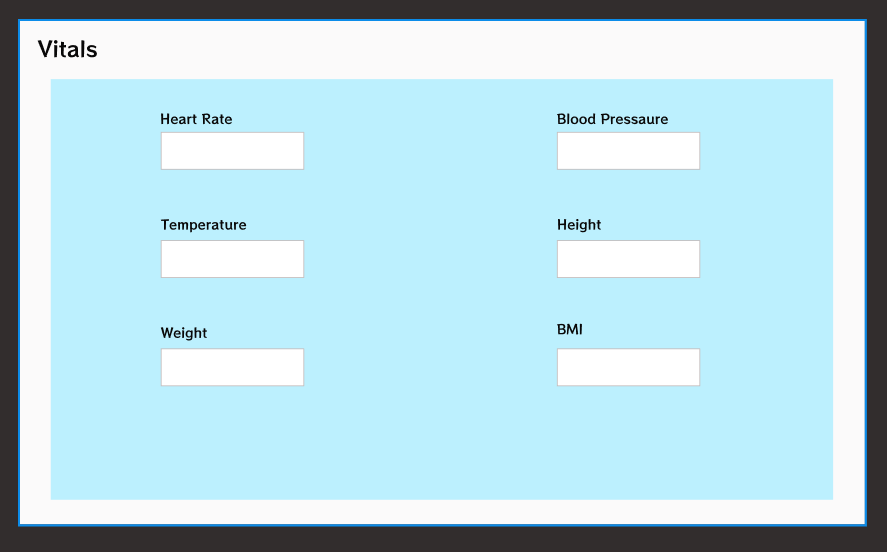
\includegraphics[height=6cm]{images03/3-2-2-figure4a.png}
    \caption{}
    \label{fig:vitals-v1}
  \end{subfigure}\hfill
  \begin{subfigure}[t]{0.48\linewidth}
    \centering
    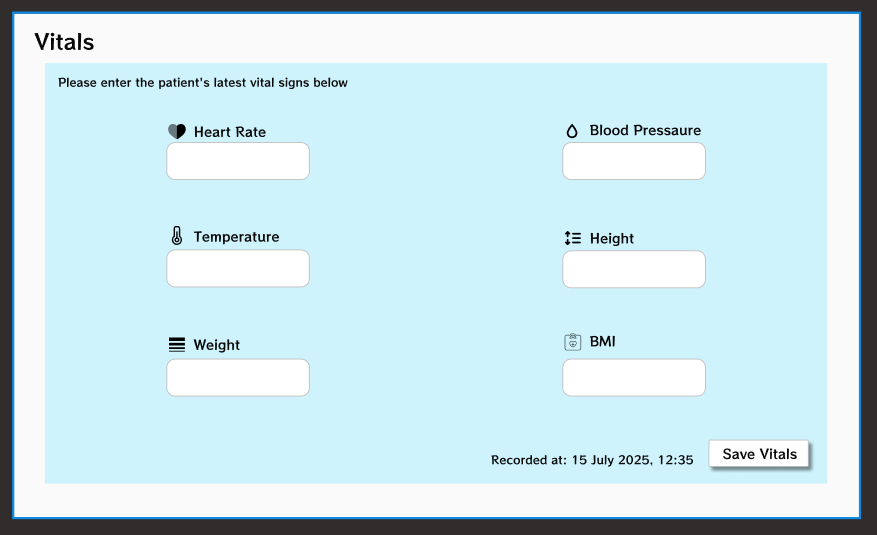
\includegraphics[height=6cm]{images03/3-2-2-figure4b.png}
    \caption{}
    \label{fig:vitals-v2}
  \end{subfigure}
\end{figure}
\begin{figure}[H]\ContinuedFloat
  \par\smallskip
  \begin{subfigure}[t]{0.48\linewidth}
    \centering
    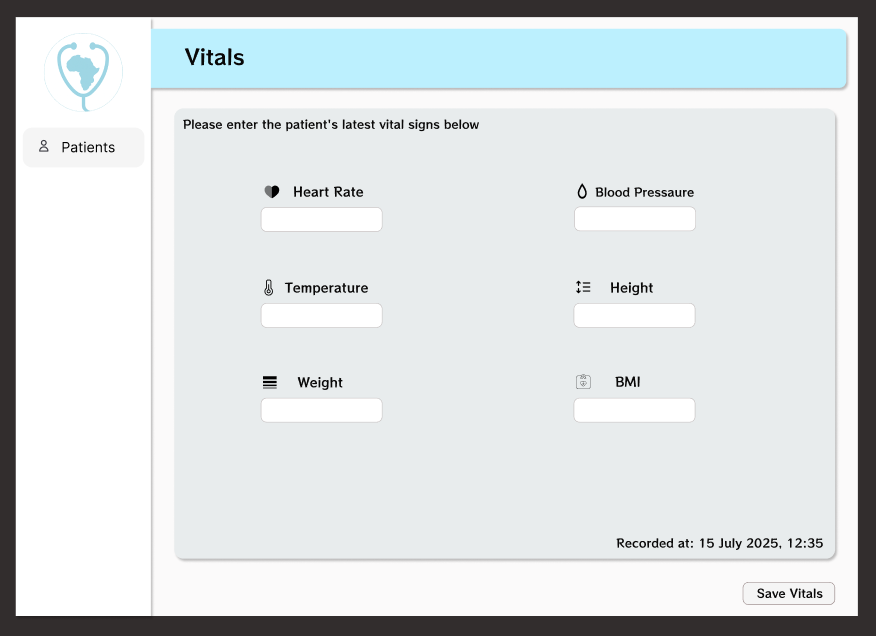
\includegraphics[height=6cm]{images03/3-2-2-figure4c.png}
    \caption{}
    \label{fig:vitals-v3}
  \end{subfigure}\hfill
  \begin{subfigure}[t]{0.48\linewidth}
    \centering
    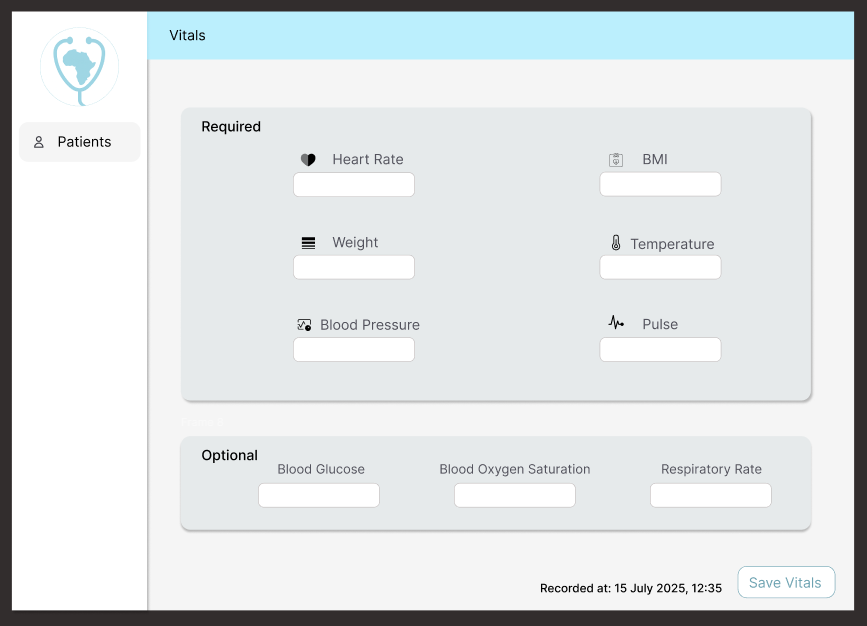
\includegraphics[height=6cm]{images03/3-2-2-figure4d.png}
    \caption{}
    \label{fig:vitals-v4}
  \end{subfigure}
\end{figure}
\begin{figure}[H]\ContinuedFloat % Part 2 of the figure
  \centering
  \begin{subfigure}[t]{0.48\linewidth}
    \centering
    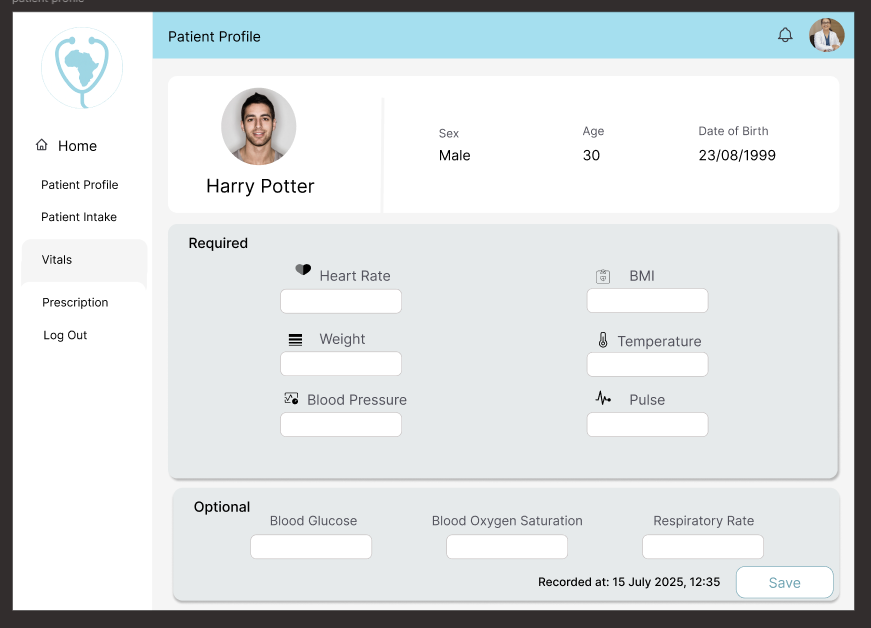
\includegraphics[height=6cm]{images03/3-2-2-figure4e.png}
    \captionsetup{justification=centering}
    \caption{}
    \label{fig:vitals-v5}
  \end{subfigure}\hfill
  \begin{subfigure}[t]{0.48\linewidth}
    \centering
    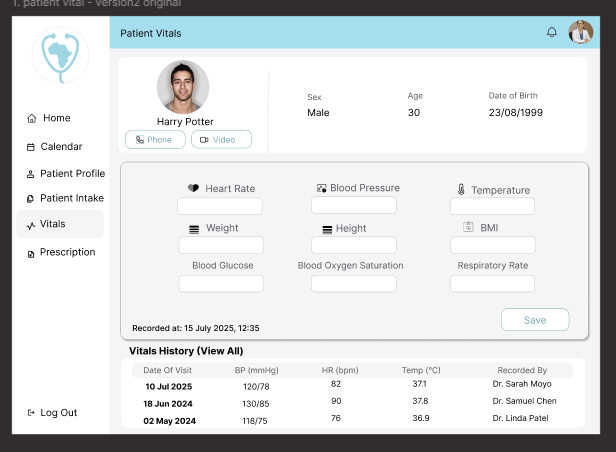
\includegraphics[height=6cm]{images03/3-2-2-figure4f.png}
    \captionsetup{justification=centering}
    \caption{}
    \label{fig:vitals-v6}
  \end{subfigure}
  %\captionsetup{justification=centering}
  \caption{The iterative design process of the Vitals page, showing its evolution through six key versions. (a) Basic layout without a sidebar or patient card. (b) Introduction of a navigation sidebar. (c) Adding a patient information card at the top. (d) Refining the layout and adding a history table. (e) Improving visual consistency and button placement. (f) Final design with all key components integrated.}
  \label{fig:vitals-evolution}
\end{figure}

These changes not only enhanced the interface visually, but also made the page much more usable in a real clinical workflow. Since healthcare professionals often move quickly between patient records, having the patient card consistently displayed at the top of all patient-specific pages helps reduce confusion, reminding them of whose data they are viewing or editing.

We made multiple adjustments to several pages based on weekly feedback from our supervisor and internal team reviews. This ensured a more user-friendly and functional design across the platform.

One of the most significant design iterations in our project involved the Prescription Page. During a weekly meeting with our supervisor, we received feedback that the initial layout appeared empty and lacked the essential clinical details typically expected in a real-world healthcare system. Based on this feedback, we conducted research into existing healthcare system standards to understand what prescription interfaces should contain, with a particular focus on NHS guidelines and clinical UX principles.

% NOTE: Please replace 'rcp_med_standards' and 'nhs_design_system' with the correct keys from your thesisbiblio.bib file.
We referred to the \emph{Medication and Allergy Standards for structured records}, published by the Royal College of Physicians in collaboration with the Health and Social Care Information Centre (HSCIC) in 2013. These standards recommend that digital prescriptions should include key information such as medication name, dosage, frequency, route, duration, and notes, all of which are fields we implemented in our updated interface~\cite{rcp_med_standards}.

In terms of user interface design, we followed the NHS Design System’s guidance on card components, which recommends grouping related form fields into visually distinct blocks. This improves usability and reduces cognitive load by allowing clinicians to focus on one section at a time. Inspired by this, we introduced structured “Medication Cards” in our interface, each containing fields for medication name, dosage (e.g., 500mg), frequency (e.g., twice a day), route (e.g., oral or IV), duration (e.g., for 7 days), and clinical notes (e.g., take before meals). We also added a dropdown for selecting saved medication records, improving both usability and completeness of the page~\cite{nhs_design_system}.

These changes transformed the original sparse interface into a more complete, user-friendly, and clinically appropriate design. They also align our application with industry standards for both content structure and interface design, as shown in Figure~{\ref{fig:prescription-evolution}}.

\begin{figure}[htbp]
  \centering
  \captionsetup[subfigure]{labelformat=simple, labelsep=space, justification=centering}
  \renewcommand{\thesubfigure}{(\alph{subfigure})}
  \begin{subfigure}[t]{0.48\linewidth}
    \centering
    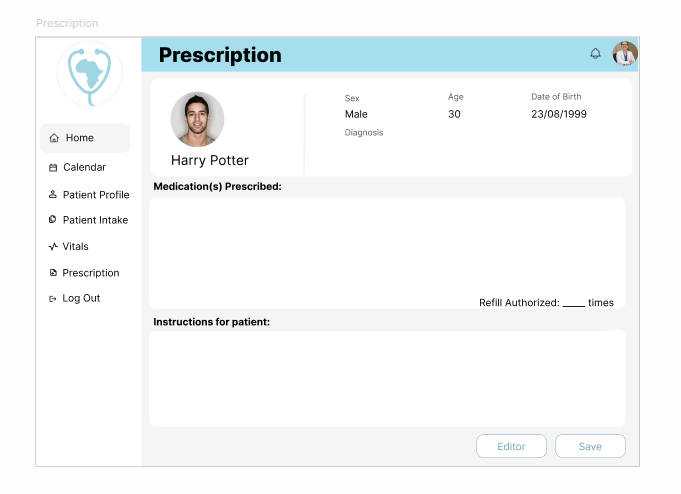
\includegraphics[height=6cm]{images03/3-2-2-figure5a.png}
    \caption{}
    \label{fig:prescription-before}
  \end{subfigure}\hfill
  \begin{subfigure}[t]{0.48\linewidth}
    \centering
    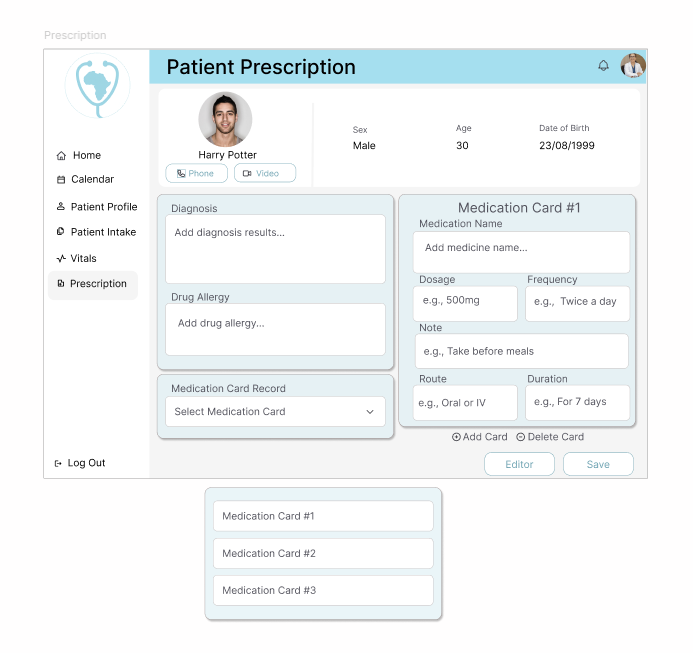
\includegraphics[height=6cm]{images03/3-2-2-figure5b.png}
    \caption{}
    \label{fig:prescription-after}
  \end{subfigure}
  \caption{Comparison of the Prescription Page before and after design iteration based on supervisor feedback. (a)Initial design of the Prescription Page. (b)Redesigned page with structured ``Medication Cards'' and comprehensive fields, following NHS guidelines.}
  \label{fig:prescription-evolution}
\end{figure}

Similarly, during one of our internal design review meetings, we identified a gap in the Patient Profile Page. Initially, the Patient Profile Page featured the doctor’s profile picture, but it lacked interactivity. In a later iteration, we enhanced the design by implementing a functional popup menu. This allowed doctors to either access their account settings or securely log out, improving both usability and navigation consistency, as shown in Figure~{\ref{fig:profile-menu-evolution}}. These feedback-driven design iterations not only improved usability but also aligned the interface with real-world clinical workflows and recognized healthcare UI standards.

\begin{figure}[H]
  \centering
  \captionsetup[subfigure]{labelformat=simple, labelsep=space, justification=centering}
  \renewcommand{\thesubfigure}{(\alph{subfigure})}
  \begin{subfigure}[t]{0.48\linewidth}
    \centering
    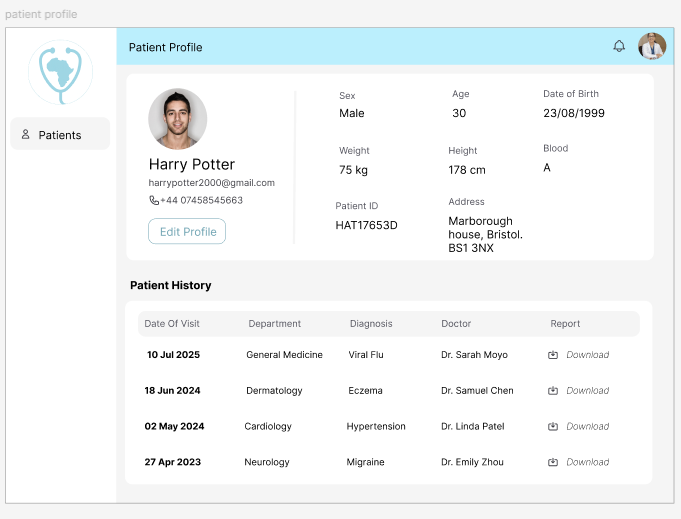
\includegraphics[height=6cm]{images03/3-2-2-figure6a.png}
    \caption{}
    \label{fig:profile-menu-before}
  \end{subfigure}\hfill
  \begin{subfigure}[t]{0.48\linewidth}
    \centering
    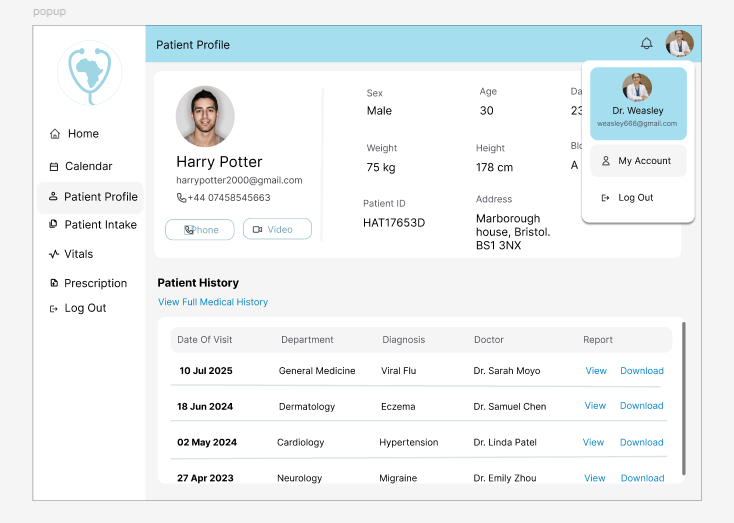
\includegraphics[height=6cm]{images03/3-2-2-figure6b.png}
    \caption{}
    \label{fig:profile-menu-after}
  \end{subfigure}
  \caption{Evolution of the doctor's profile menu on the Patient Profile Page. (a)Initial design with a static, non-interactive doctor profile picture. (b)Enhanced design with a functional popup menu for account settings and logout.}
  \label{fig:profile-menu-evolution}
\end{figure}



\paragraph{Front-end Implementation}\mbox{}\\

In the front-end implementation section, we illustrate the process of how we created, organised, and tested our front-end code. We divide this process into 5 stages. First, we describe how we structured and developed the codebase. Then, we explain how we integrate shared layouts using Thymeleaf to improve consistency and maintainability across pages. Next, we explain how different pages are connected to form a smooth user flow. We also discuss the steps we took to test each function to ensure the website behaves as intended. Finally, we reflect on the main challenges we encountered during the front-end development and how we addressed them. These topics are covered in following subsections: Code Structure and Component Organisation, Integrating Shared Layouts with Thymeleaf, Page Navigation and User Flow, User Flow and Functional Testing, and Challenges Encountered During Frontend Development, respectively.
\paragraph{Code Structure and Component Organisation}\mbox{}\\
In this section, we describe how we constructed the front-end codebase. As mentioned earlier, each member was responsible for designing different parts of the website in Figma. We continued the pattern during implementation–each member developed their assigned parts using HTML and CSS, focusing on accurately reproducing the layout and visual style from our Figma design.

At this stage, our goal is to replicate the layout and visual style of our Figma design. Most interactive elements, such as buttons, pop-up windows, and form submissions, have not yet been functionalized. We have also not yet integrated a shared layout system using Thymeleaf. These shared elements are currently duplicated across individual pages, and we plan to organize them in the next development stage to improve maintainability and consistency.

\paragraph{Integrating Shared Layouts with Thymeleaf}\mbox{}\\
After developing all the pages, we noticed that many structural elements–such as headers, sidebars, and forms–were repeated across different pages. To reduce redundancy and to make the Smart Hospital UI consistent and maintainable, we wrapped repeated interface components (sidebar, top navigation, and patient header) into reusable Thymeleaf fragments and consumed them across pages with th:replace. As shown in Figure~\ref{fig:3-2-2-vital-history-page}, the vitalsHistoryPage.html file defines an empty container, CSS links, outer grid, and main content area, while common UI components are injected at render time from layouts/sharedLayout.html.

\begin{figure}[H]
  \centering
  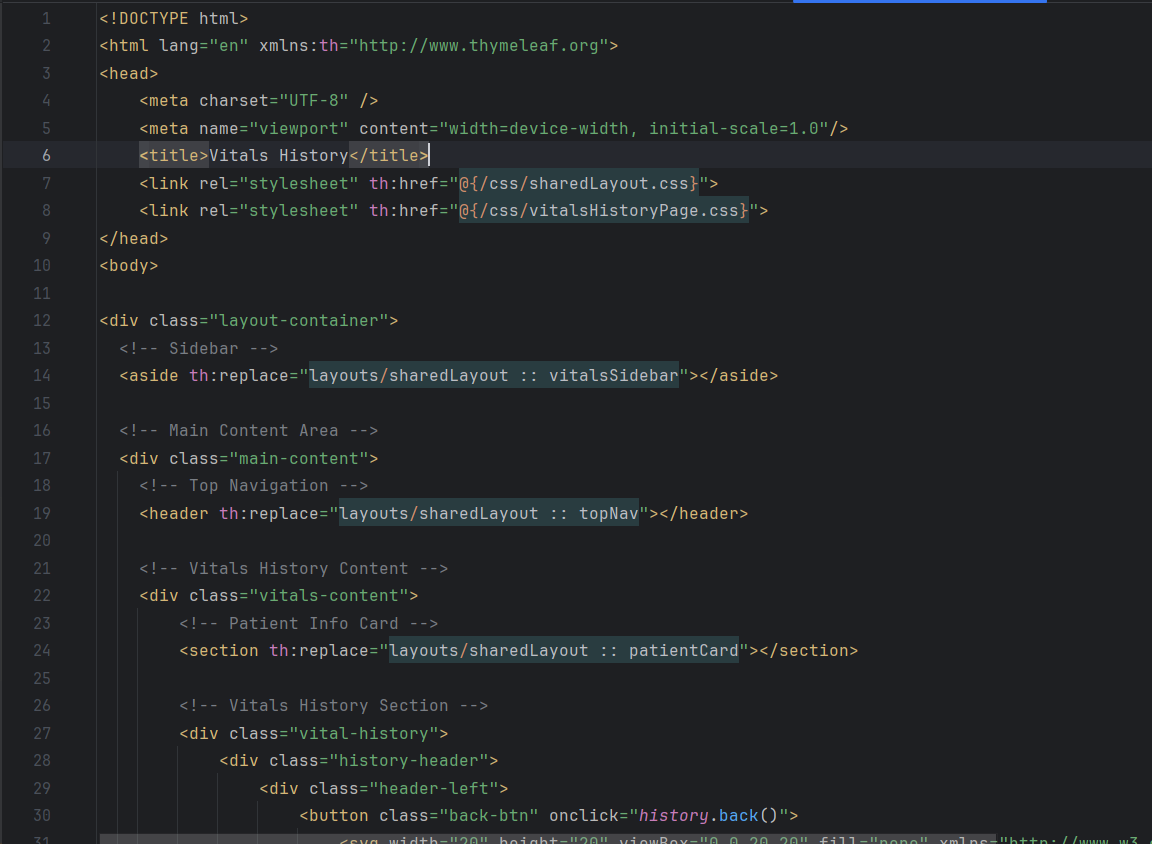
\includegraphics[width=0.8\linewidth]{images03/3-2-2-vitalHS.png}
  \caption{vitalsHistoryPage.html consuming shared fragments (vitalsSidebar, topNav, patientCard) via th:replace.}
  \label{fig:3-2-2-vital-history-page}
\end{figure}

For example, the Vitals page loads the active vitalsSidebar fragment (highlighting the Vitals tab), the topNav fragment (with dynamic pageTitle provided via the model), and a patientCard fragment (so clinicians can always see the patient context at the top of patient-specific pages). This server-side composition makes our design system dry, updating the sidebar icon set or the patient header once applied everywhere without touching individual pages. Figure~\ref{fig:3-2-2-sharedLayout} illustrates part of the sharedLayout.html file, displaying the sidebar fragment and its logo and most crucial navigation links.

\begin{figure}[H]
  \centering
  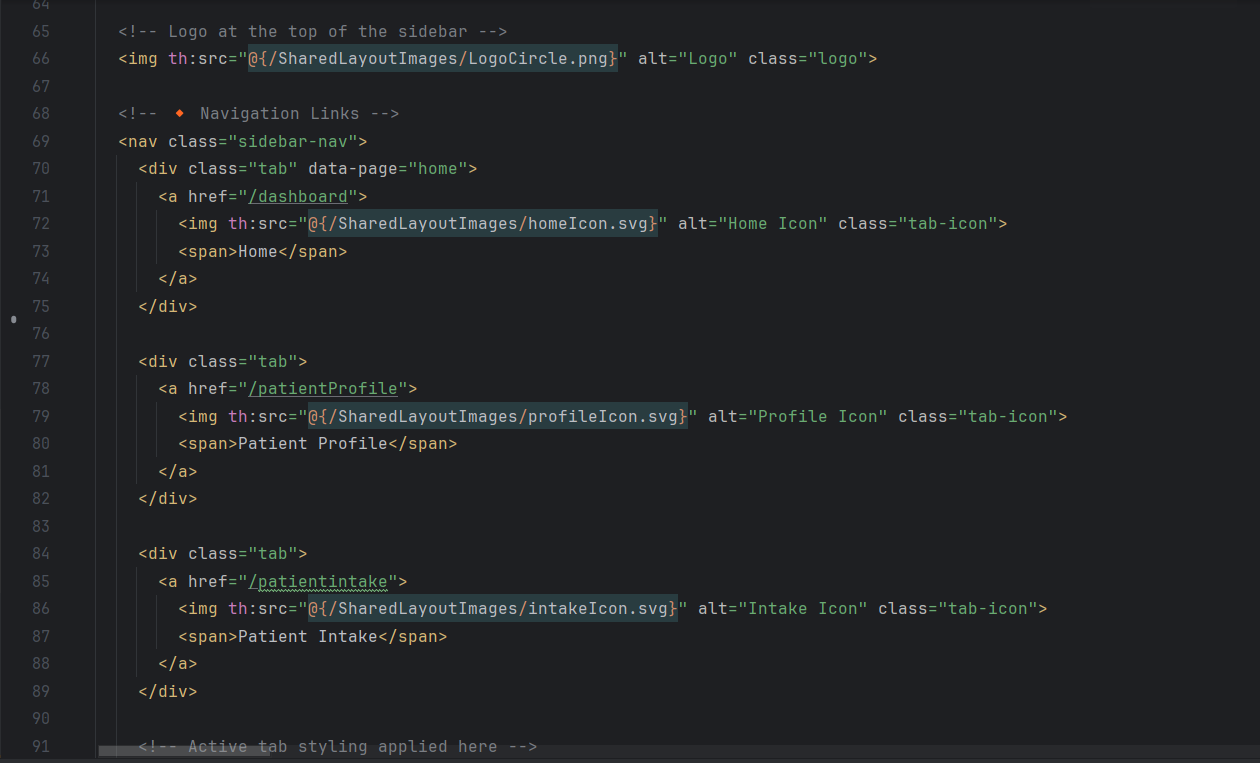
\includegraphics[width=0.8\linewidth]{images03/3-2-2-sharedLayout.png}
  \caption{Snippet from sharedLayout.html showing the sidebar fragment, including the logo at the top and navigation links.}
  \label{fig:3-2-2-sharedLayout}
\end{figure}

We also separated shared and page-specific styling concerns to avoid cascade conflicts. Fragment-level styles for global pages live in \verb|sharedLayout.css| and are loaded ahead of each page's own stylesheet (e.g., \verb|vitalsHistoryPage.css|). Fragments leverage Thymeleaf's URL syntax (e.g., \verb|th:src="@{/SharedLayoutImages/}"|) to refer to assets so paths get resolved properly no matter the environment. Where a page needs alternative "active" navigation, we provide a purpose-specific fragment (e.g., \verb|sidebar| vs. \verb|vitalsSidebar|) to facilitate correct tab state without hardcoded per-page logic. This approach assisted in achieving consistency (the same chrome everywhere), maintainability (one change affects all pages), and clarity. As shown in Figure~\ref{fig:3-2-2-renderLayout}, clinicians always have navigation context and the patient card visible when navigating between modules.

\begin{figure}[H]
  \centering
  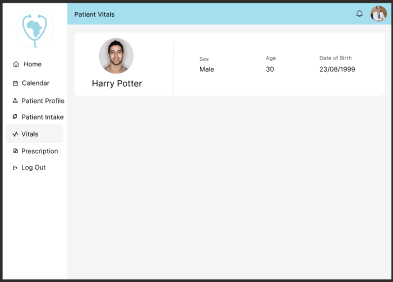
\includegraphics[width=0.8\linewidth]{images03/3-2-2-renderLayout.png}
  \caption{Rendered UI in the browser showing the shared sidebar, patient card, and top navigation in the Vitals module.}
  \label{fig:3-2-2-renderLayout}
\end{figure}

\paragraph{Page Navigation and User Flow}\mbox{}\\
In this stage, we began to functionalize interactive elements such as buttons, hyperlinks to ensure the website provides a smooth and intuitive experience. The overall user flow had already been defined in our early-stage Figma design, a clear user flow that reflects typical interactions between patients and doctors in our early-stage Figma design, reflecting typical interactions between patients and doctors. Each page was connected according to the logical steps users would take when navigating through the platform. For example, clicking the “Register” button on the homepage directs users to the registration form, and buttons on the “Dashboard” page are linked to corresponding pages. These workflows were clearly visualized in our Figma prototype. The main goal of this stage is to ensure that all the interactive elements function as the origin design. In the next stage, we plan to test the whole website work appropriately and collect the disadvantages that can be improved.
\paragraph{User Flow and Functional Testing}\mbox{}\\

\paragraph{Challenges Encountered During Frontend Development}\mbox{}\\
One of the biggest challenges encountered while performing frontend development was how to break down the Figma-based design system into Thymeleaf templates. Even though the Figma designs created a solid visual reference for layout, typography, and spacing between elements, the server-side rendering approach of Thymeleaf required the interface to be split into smaller, more manageable parts. It introduced additional difficulty in the process of converting pixel-perfect designs into coherent HTML templates with alignment, responsiveness, and style consistency preserved. Visual parity usually needed to be delivered by iterative adjustments of the HTML structure as well as accompanying CSS.

An analogous problem involved the handling of shared styles and bits within the multi-page Thymeleaf application. Shared interface pieces, the sidebar navigation, header, and footer, were included as reusable fragments to foster consistency and reduce redundancy. With this came, however, the risk of side effects: a modification of a shared fragment would likely disrupt the styling or layout of multiple pages. To tackle this, the development team implemented a formalized update process, such as fragment-specific testing and peer review prior to merge of changes. This procedure ensured global component updates maintained visual correctness without causing regressions in other parts of the system.


\section{Back-end Design and Implementations}
\label{sec:sec03}
